\chapter{系统需求分析}

本章主要对基于TIL-STD-6016数据链信息标准数据库与应用平台进行系统需求分析,确定系统的功能需求和非功能需求,为后续的系统设计与实现提供依据。

战术数据链系统是当前联合作战中通信手段中最基础的通信手段,信息标准数据库是提高作战效能,增强系统互操作能力的关键。随着网络中心战概念的提出和发展,对多域作战需求,传统战术数据链系统数据繁杂,版本标准不一,多链路间互操困难等问题越来越明显,构建一个统一的、高效的、可扩展的战术数据链信息标准数据库系统是当前军事信息建设的新方向。

本章将基于系统需求分析角度描述基于MIL-STD-6016标准的战术数据链信息标准数据库系统的功能需求、非功能需求、数据特征与处理需要、用户角色与交互需求,根据以上系统的信息需求,对后期系统架构设计、系统数据库建模、系统前后端开发与系统集成测试提出需求与约束。

\section{功能需求}

根据前期调研和标准分析,结合实际应用场景,系统需要实现以下核心功能:

\subsection{数据特征与处理需求}
战术数据链消息具有与传统业务数据不同的特性,其处理需求也更为复杂。为保证数据库的适用性与系统的实用性,需从数据来源、结构特征、处理方式与存储管理等角度加以分析\cite{baek2016_jsac}。

系统数据主要来源于 {MIL-STD-6016}、{MIL-STD-3011}、{STANAG-5516} 等标准文档,并结合 {MAVLink}、{NMEA-0183}、{ARINC-429} 等协议数据。数据类型主要包括:

(1)标准消息数据:J 系列报文(J2.0、J3.0、J7.0、J12.0等)及其字段定义;

(2)语义概念数据:基于CDM四层法的概念库和字段映射关系;

(3)多格式文档数据:PDF、XML、JSON、CSV等格式的标准文档和配置文件;

(4)跨协议转换数据:不同协议间的消息转换和映射规则。

表\ref{table_data_features}详细展示了战术数据链数据特征与处理需求的对应关系,该表从数据类型、结构特点、处理需求和存储实体四个维度进行了系统性的分析。

\begin{table}[!htb]
    \caption{战术数据链数据特征与处理需求概览}
    \label{table_data_features}
    \centering
    \adjustbox{width=0.9\textwidth,center}{%
    \begin{tabular}{lccc}
        \hline
        \textbf{数据类型} & \textbf{结构特点} & \textbf{处理需求} & \textbf{存储实体} \\
        \hline
        标准消息数据 & 多字段/比特位 & 报文解析、完整性校验 & 消息表、字段表 \\
        语义概念数据 & 概念层次/同义映射 & 概念绑定、语义一致性 & 概念表、绑定表 \\
        多格式文档数据 & 格式多样/结构复杂 & 多格式解析、智能识别 & 文档表、解析结果表 \\
        跨协议转换数据 & 格式差异/协议适配 & 格式转换、协议映射 & 映射表、转换规则表 \\
        \hline
    \end{tabular}%
    }
\end{table}


\subsection{标准消息管理}
战术数据链信息标准数据库系统需要支持多种消息标准的统一管理\cite{CurtissWright_TCG_HUNTR_2020}。根据实际应用需求分析,系统应具备以下核心能力:

(1)多标准消息支持:系统需要同时支持MIL-STD-6016的J系列消息(J2.0、J3.0、J7.0、J12.0等)、MAVLink的飞行器通信消息(HEARTBEAT和ATTITUDE、VERSAGE、ATTIME)、NMEA-0183的导航消息(GGA、RMC和VTG等),每一种消息都具有特定的格式、语义和适用范围,系统要能够完整地存储管理消息的定义信息(消息基本信息、消息结构、消息语义信息)。

系统支持的标准和协议如下表\ref{table_supported_standards}所示。


\begin{table}[!htb]
    \caption{系统支持的标准和协议}
    \label{table_supported_standards}
    \centering
    \adjustbox{width=0.9\textwidth,center}{%
    \begin{tabular}{lccc}
        \hline
        \textbf{标准名称} & \textbf{描述} & \textbf{版本} & \textbf{主要消息类型} \\
        \hline
        MIL-STD-6016 & 美军标准6016 - 战术数据链消息标准 & A, B, C & J2.0, J3.0, J7.0, J12.0, J13.0 \\
        MIL-STD-3011 & 美军标准3011 - 联合战术信息分发系统 & A, B & J2.0, J2.2, J3.0, J3.1, J3.3 \\
        STANAG-5516 & 北约标准5516 - 战术数据交换 & 1, 2, 3 & J2.0, J3.0, J7.0, J12.0 \\
        MAVLink & 微型飞行器通信协议 & 1.0, 2.0 & HEARTBEAT, ATTITUDE, POSITION, GPS\_RAW\_INT \\
        NMEA-0183 & 海洋电子设备数据格式 & 2.0, 2.1, 2.2, 2.3 & GGA, RMC, VTG, GLL, GSA \\
        ARINC-429 & 航空电子设备数字信息传输 & 15, 16, 17 & A429, A629 \\
        \hline
    \end{tabular}%
    }
\end{table}

(2)消息录入与维护:考虑到标准文档的复杂性和多样性,系统需要支持多种数据录入方式。传统的逐条录入方式效率低下,无法满足大规模标准文档的处理需求。系统需要提供基于PDF文档的自动化解析功能,能够从标准文档中自动提取消息定义信息,并支持CSV、Excel、XML、JSON等多种格式的批量导入和单个录入两种方式。

(3)消息字段管理:J系列消息复杂,消息字段由字段名、起始位置、结束位置、长度、描述信息等属性组成,系统应能支持复杂字段管理并建立字段与消息的绑定关系;系统应能支持字段层次管理,支持字段组、子字段等,便于管理和理解消息。


\subsection{字段与语义概念绑定}
为提升消息语义一致性,系统需要支持字段与语义概念的绑定\cite{Chelton_Link16_Antennas_2022}。根据实际应用需求分析,系统应具备以下核心能力:

(1)语义概念库构建:需建立统一的语义概念库,包含战术数据链领域中的核心概念,如平台标识、位置信息、时间信息、任务状态等。每个语义概念都应具有明确的定义、属性描述和使用规则,支持概念的层次化组织和继承关系。

(2)字段绑定机制:系统需要支持自动绑定和手动绑定两种方式。自动绑定基于字段名称、数据类型、取值范围等特征进行匹配,能够快速建立初步的绑定关系。手动绑定允许专家用户根据领域知识进行精确的绑定操作,确保绑定的准确性和完整性。

(3)置信度管理:在功能上需要为每个字段-概念绑定关系分配置信度值,反映绑定的可靠程度。置信度可以通过字段名称相似度、数据类型匹配度、专家验证结果等因素计算,并提供置信度阈值设置功能,允许用户根据应用需求调整绑定标准。

(4)动态绑定更新:考虑到战术数据链标准的不断演进,应支持语义绑定的动态更新,当标准版本更新或新增消息类型时,能够自动检测需要重新绑定的字段,并提供批量更新功能。

\subsection{多链路互操作支持}
考虑到战术数据链存在多标准并行的情况,系统需要具备跨链路的互操作支持功能\cite{AFCEA_Link16_Improvements_2022}。根据实际应用需求分析,系统应具备以下核心能力:

(1)CDM四层法架构:系统需采用CDM(Common Data Model)四层法架构实现多协议互操作。概念层定义统一的语义概念库,包含作战实体、态势要素、指挥关系等核心概念;映射层通过声明式规则定义协议间的字段映射关系;转换层实现具体的消息转换逻辑;运行层提供协议中介和转换引擎。系统支持MIL-STD-6016、MAVLink、MQTT、NMEA-0183等协议的互操作转换,这种分层架构确保系统的可扩展性和可维护性。

图\ref{fig_cdm_architecture}展示了CDM四层法架构,包括语义层(统一概念库)、映射层(YAML配置规则)、校验层(一致性验证)和运行层(转换引擎),展现了多协议间的语义互操作和实时转换。

\begin{figure}[H]
    \centering
    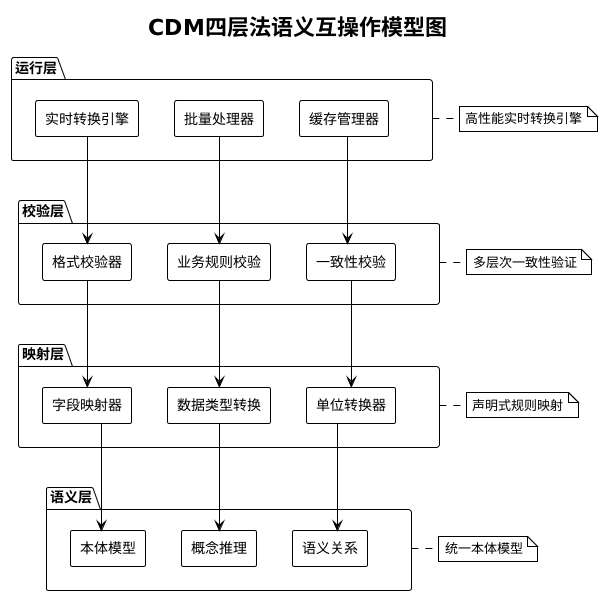
\includegraphics[width=0.6\textwidth,height=0.5\textheight,keepaspectratio]{chapters/fig-0/cdm_four_layer_simple.png}
    \caption{CDM四层法架构图}
    \label{fig_cdm_architecture}
\end{figure}

(2)智能消息转换引擎:应实现基于规则和机器学习的智能转换引擎,能够自动处理协议间的语法差异、语义差异和时序差异。转换引擎需要支持多种转换策略,包括精确匹配、模糊匹配、语义推理等,并提供转换质量评估和置信度评分机制。

(3)统一API网关:需提供统一的API网关,支持多种协议的消息转换和路由。网关需要集成CDM四层法和语义互操作两种处理方式,能够根据源协议和目标协议自动选择最优的转换策略。
下表\ref{table_api_interfaces}列出了系统提供的5个主要API接口及其功能,通过RESTful架构设计为前端界面和外部系统提供标准化数据交换接口。

\begin{table}[!htb]
    \caption{系统API接口功能表}
    \label{table_api_interfaces}
    \centering
    \adjustbox{width=0.9\textwidth,center}{%
    \begin{tabular}{lccc}
        \hline
        \textbf{API接口} & \textbf{主要功能} & \textbf{支持格式} & \textbf{应用场景} \\
        \hline
        /api/v2 & 消息转换、概念管理、映射管理、系统统计 & JSON, XML & 统一文档处理与语义互操作 \\
        /api/cdm & CDM概念创建、映射规则管理、消息转换 & JSON, YAML & CDM四层法互操作处理 \\
        /api/semantic & 语义字段管理、消息映射、路由处理 & JSON, XML & 语义互操作系统 \\
        /api/pdf & PDF文档解析、表格提取、数据处理 & PDF, JSON & MIL-STD-6016文档处理 \\
        /api/mqtt & MQTT消息处理、协议转换、数据路由 & JSON, MQTT & MQTT协议消息处理 \\
        \hline
    \end{tabular}%
    }
\end{table}

(4)协议适配支持:功能设计上应支持MIL-STD-6016、MAVLink、MQTT、NMEA-0183、ARINC-429等多种协议的消息对接,能够处理不同协议间的消息格式差异、语义差异和时序差异。通过声明式映射规则和版本治理机制,系统需要能够灵活应对协议演进和标准更新。


\subsection{前端交互与可视化}
基于前述数据库操作与维护的需求,战术数据链信息标准数据库系统面向的用户群体包括系统管理员、作战指挥员、研发人员等,这些用户具有不同的技术背景和使用需求,因此前端系统应具备以下核心能力:

(1)统一用户界面:需提供统一文档处理与语义互操作平台,包含消息处理、文件处理、概念管理、映射管理、系统概览等核心功能模块,支持用户通过消息号、字段名、J系列类别、时间范围等多种条件进行精确查询,并支持查询条件的保存和重用,允许用户创建常用的查询模板。

(2)数据展示与搜索:应支持多种数据展示方式,包括表格、图表、关系图等,其中表格展示需支持排序、筛选、分页等功能,并提供数据导出能力,图表展示应支持多种图形显示方式(包括条形图、饼状图、折线图等),让用户直观地了解数据的分布与趋势。另外,应支持智能搜索引擎,提供模糊匹配、语义搜索等功能,使用户能够便捷地找到所需要的信息。

(3)交互式操作:为确保良好的用户体验和系统可用性,需支持交互式操作和响应式设计。系统应支持拖拽、点击、缩放等交互操作,允许用户通过直观的手势操作来浏览和操作数据,并提供上下文菜单、快捷键等便捷操作方式,提高用户的操作效率。

系统需针对不同用户提供差异化的交互模式\cite{reid_2018_nav_leo}:

(1)图形化交互:前端界面提供消息检索、态势展示和跨链协议映射的可视化操作,支持CDM互操作接口、语义互操作接口和统一处理器接口,降低使用门槛,如图\ref{fig_usecase_frontend}所示。
% ================= 新增:用例图 =================
\begin{figure}[H]
    \centering
    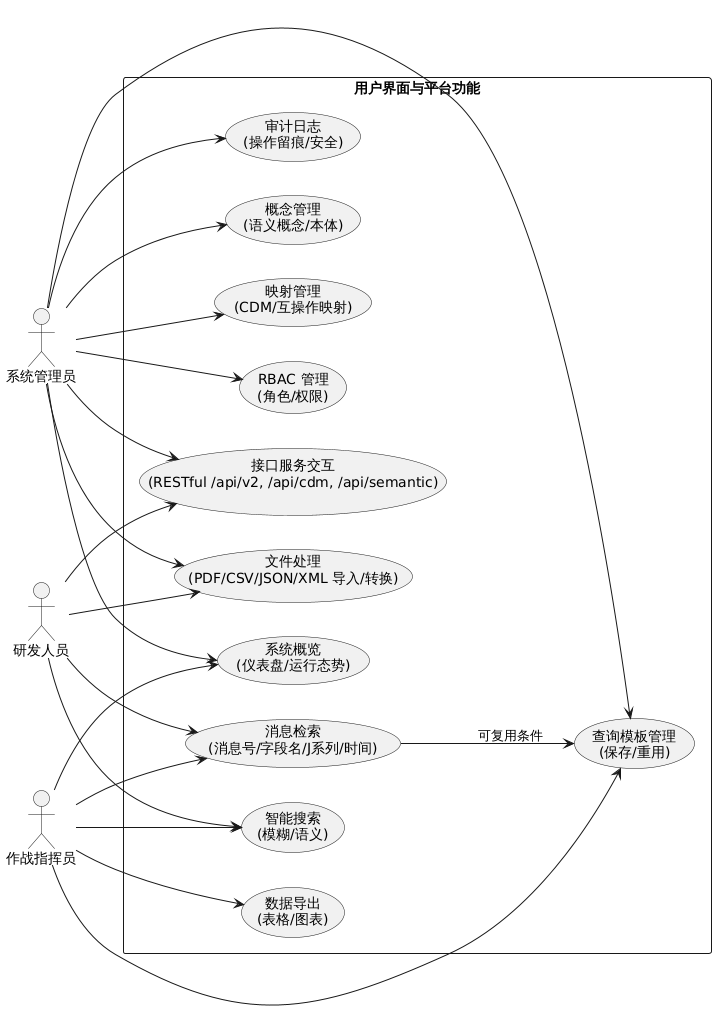
\includegraphics[width=0.8\textwidth,height=0.5\textheight,keepaspectratio]{chapters/fig-0/usecase_frontend.png}
    \caption{前端交互用例图(角色与功能关系)}
    \label{fig_usecase_frontend}
  \end{figure}
(2)命令行接口:为研发与仿真人员提供批处理与脚本化调用,支持大规模数据处理与自动化测试。

(3)接口服务交互:通过 RESTful API 与外部仿真平台或作战系统对接,支持标准化协议调用和跨域互操作,提供/api/v2、/api/cdm、/api/semantic等统一API接口,如图\ref{fig_component_frontend} 所示。



% ================= 新增:组件图 =================
\begin{figure}[H]
  \centering
  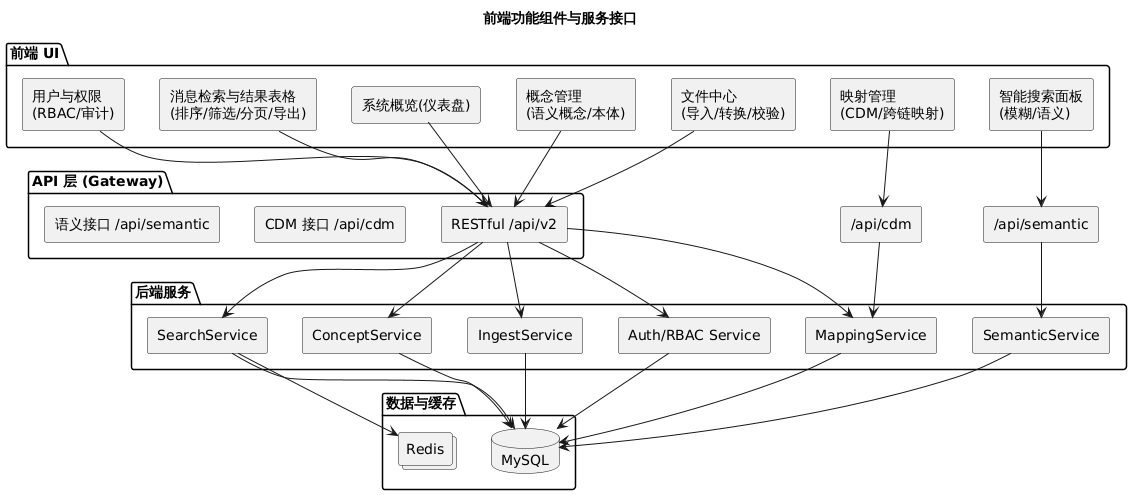
\includegraphics[width=0.8\textwidth,height=0.6\textheight,keepaspectratio]{chapters/fig-0/component_frontend.png}
  \caption{前端功能组件与服务接口关系图}
  \label{fig_component_frontend}
\end{figure}


\subsection{仿真与验证接口}
作为战术数据链验证和测试的输入源,高质量的仿真数据当然不可或缺;而高质量的仿真平台同样离不开可靠的消息定义和消息格式,所以系统需要构建高可用的仿真/数据接口。

而对于面向接口,需要系统提供标准的面向接口(RESTful API)实现,能够支撑仿真平台的数据获取、消息发送、结果获取等基本操作;接口实现为标准的 HTTP 实现,定义状态码,接口易于维护,可支持多种标准的消息格式类型(JSON,XML,YAML);消息格式定义了消息结构、字段、语义信息等,仿真平台可基于此对消息内容做出正确的理解与处理。

\section{系统非功能性需求分析}

作为保障作战指挥的信息系统,战术数据链数据库与应用平台还需要具备较好的非功能性,即平台除开功能性需求外,需具备良好的非功能性、可扩展性、安全性,保障平台在复杂作战环境下的正常使用及系统的发展扩展\cite{Kagioglidis_2009}。

\subsection{性能需求}
基于战术数据链系统的实时性特征和作战指挥的时效性要求,系统性能需求分析应从响应时间、数据吞吐量和系统可靠性三个维度进行考量\cite{Kee_2008,baek2016_adhoc,baek2019_jsyst_timemirror}。响应时间需求分析表明,多用户并发访问场景和实时态势更新的业务需求对系统响应性能提出了严格要求。通过分析战术数据链消息解析与字段检索的快速响应要求,可以确定普通查询请求的平均响应时间应控制在2秒以内,这一指标直接影响作战指挥的决策效率。为满足上述性能要求,系统需要实现缓存机制,包括Redis缓存和查询结果缓存,对于频繁访问的消息类型和字段定义实现预加载策略,同时建立数据库索引支持多条件组合查询的快速执行。

而对吞吐量的需求要求系统能够支持大批量数据的导入导出,以便进行标准文档与系统初始化的批量处理,通过对仿真测试场景下对数据处理的要求分析,可以得到仿真接口需要支持连续处理大量并发消息,支持消息实时生成与回放,满足仿真测试中大批量数据处理需求\cite{lee2018_jsyst,Spyridis_2010,Kopp_Throughput_Enhanced_JTIDS_2006,Juarez_2025}。对系统可靠性需求分析,复杂、不确定的战术环境要求系统容错和数据一致性,通过对数据安全性和一致性需求分析,可以得到对于数据库的要求是支持备份和日志恢复,确保异常下数据的安全,消息存储和语义绑定过程的事务一致性约束对于系统可靠性要求较高,避免不一致\cite{Koromilas_2009,EverythingRF_STT}。

\subsection{安全性需求}
战术数据链系统承载着敏感的作战数据,安全性是系统的首要需求,系统在数据存储、传输、访问控制等方面都有基本的要求,确保系统内信息不被篡改、泄露和非法窃取\cite{Collins_TTNT_immersion_2020}。系统在数据存储、数据传输方面采用加密技术,在数据库级别将敏感字段加密存储,在系统接口采用基于TLS/SSL的安全传输协议,防止中间人接入,消息交换采用密钥管理机制,密钥定期更换,防止密钥泄露\cite{Euromids_2025_contract}。

为防止非法访问与误操作,需要建立访问控制机制,提供基于角色的访问控制(RBAC),不同用户角色具备不同权限范围,对数据库的读写操作需进行身份认证与授权,提供日志审计功能,记录用户操作轨迹,便于事后追溯\cite{GovConWire_Euromids_2025}。系统应提供数据校验与完整性验证机制(如哈希校验),在通信中断或错误发生时,系统可通过重传机制与数据恢复策略保证一致性\cite{musumeci_2014_ietrsn_pulseblank,borio_2013_ietspr_pulseblanking,houdzoumis2009_jn,wu_2016_taes_dme_wp,huo_2015_ieeecl_meb,huo_2015_comex_mixed_interference,mitch_2016_nav_chirp_geolocation,vandermerwe_2023_nav_mpanf}。

\subsection{可扩展性需求}
根据战术数据链标准和作战样式发展趋势,应能够适应标准、吸收协议、拓展构架,这也是系统扩展性需求分析需要考虑的三个层次\cite{CJCS_Manuals_Library}。适应标准需求分析表示应适应标准不同版本以及NATO STANAG扩展,考虑MIL-STD-6020/STANAG5602等互操作标准的发展,应该有新接口/协议快速接入能力、数据库设计为块状的可扩展设计并支持新消息类型、新字段、新语义映射,应能够适应标准版本变化等内容\cite{CJCS_Instructions_Library,ASSIST_3011_2023}。

而根据协议融合需求分析,多链路并用的跨域作战场景下,需要融合不同链路的数据协议,通过对当前TTNT、JREAP等新兴数据链发展趋势进行梳理,确定系统架构应留有拓展接口、提供适配层、满足不同链路的不同数据结构映射和不同消息语义\cite{ASSIST_6020_2025,qin2013_gpssol}。从架构扩展需求分析,系统整体架构应能够适应未来规模化、复杂化应用场景要求,通过对微服务架构和模块化设计架构优势梳理,确定后端应基于微服务架构按需部署、前端应支持模块化扩展便于新型可视化/交互模块部署、数据库应支持可扩展结构、数据支持分片/多节点扩展\cite{fried_loeliger1979_navigation},提供接口统一支持与外界互联、采用RESTful API协议便于外部仿真平台/指挥信息系统接入、提供统一标准数据交换格式(如JSON、XML)便于与异构系统交互、提供API文档/开发者支撑便于未来扩展/二次开发\cite{baruffa2013_jsps}。